\chapter{Diseños individuales para la iteración competitiva de Dunia Namour Doughani}
\label{ape:disenyoDunia}

  En este apéndice se muestran los diseños individuales realizados por Dunia Namour Doughani para la iteración competitiva.

  \begin{figure}[ht!]
    \centering
    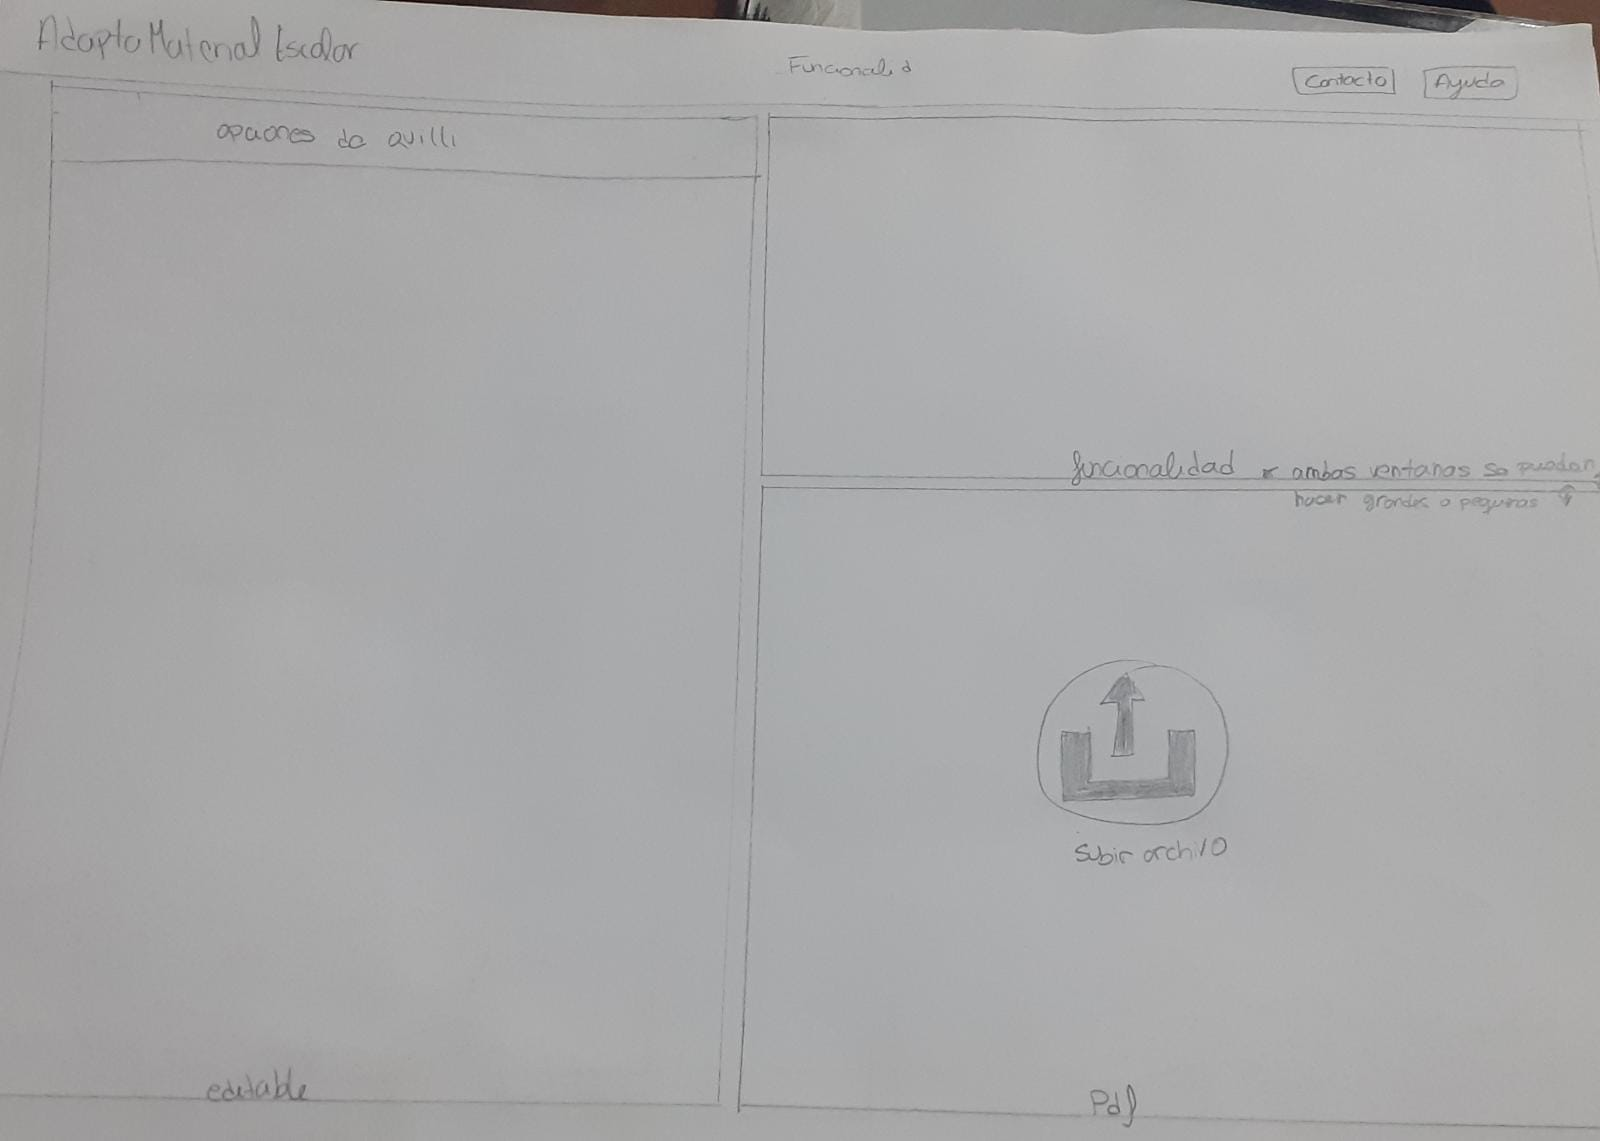
\includegraphics[width=0.6\textwidth]{Diseño/Dunia/principal.jpeg}
    \caption{Diseño pantalla de inicio de Dunia.}
    \label{dunia1}
  \end{figure}

  \begin{figure}[ht!]
    \centering
    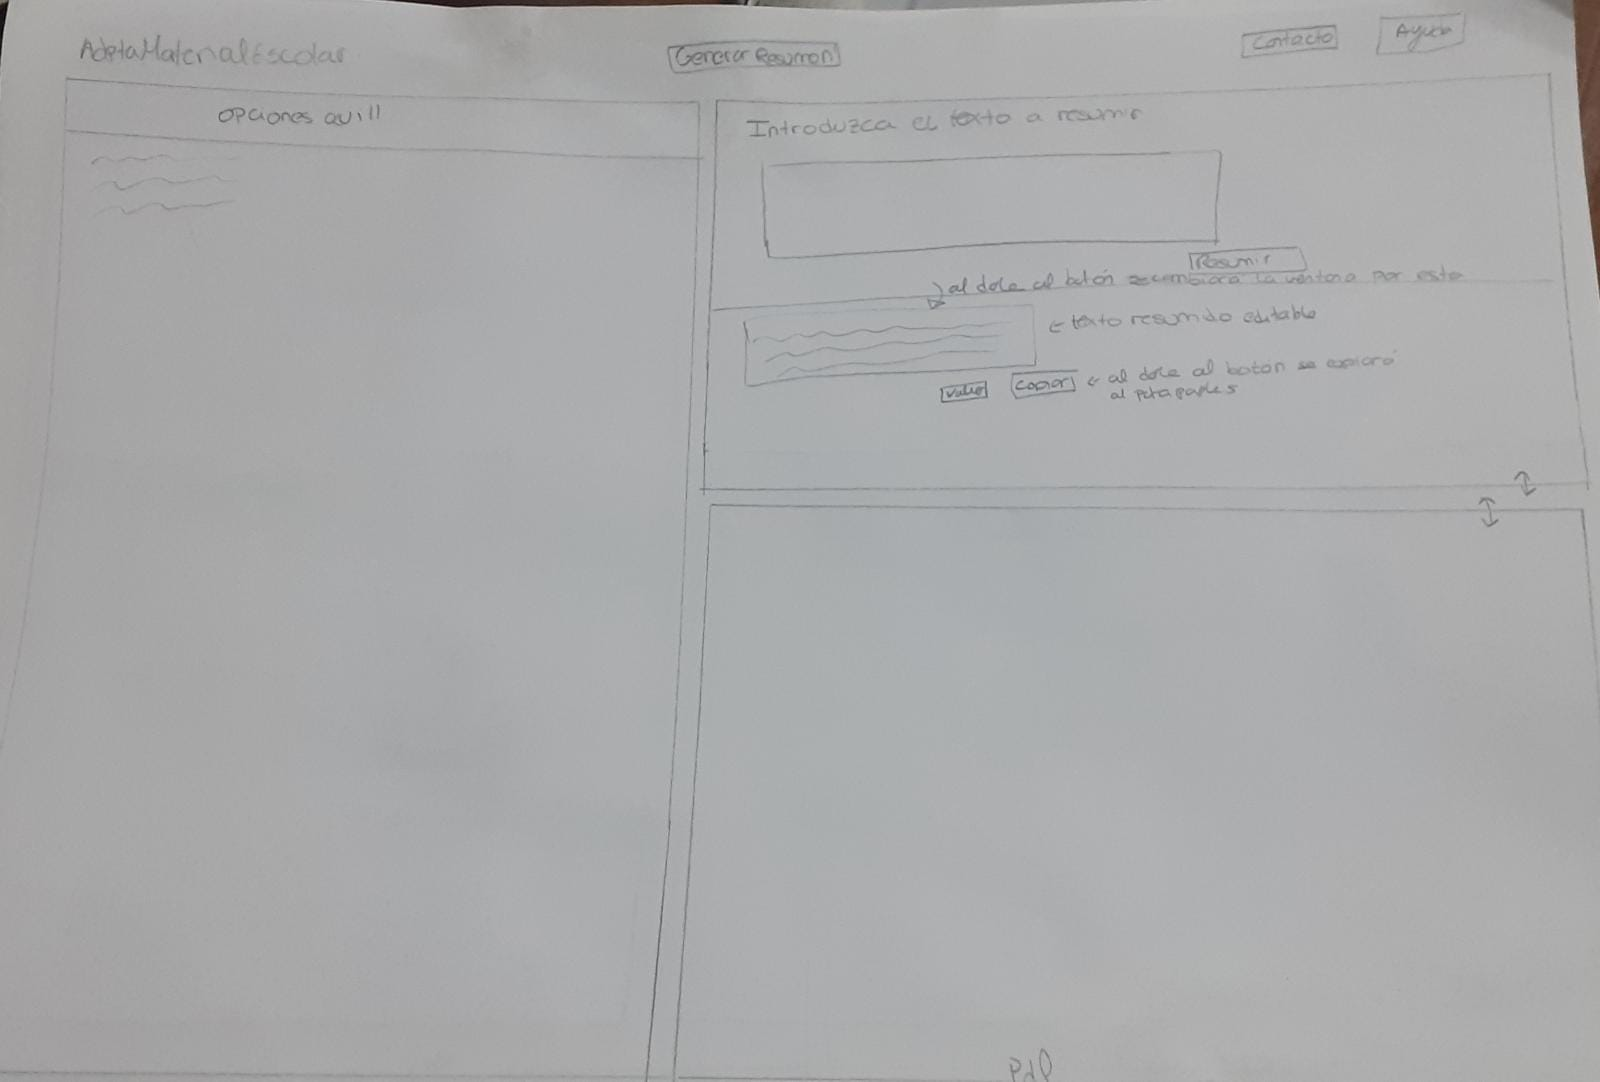
\includegraphics[width=0.6\textwidth]{Diseño/Dunia/resumen.jpeg}
    \caption{Diseño pantalla de generar resumen de Dunia.}
    \label{dunia2}
  \end{figure}

  \begin{figure}[ht!]
    \centering
    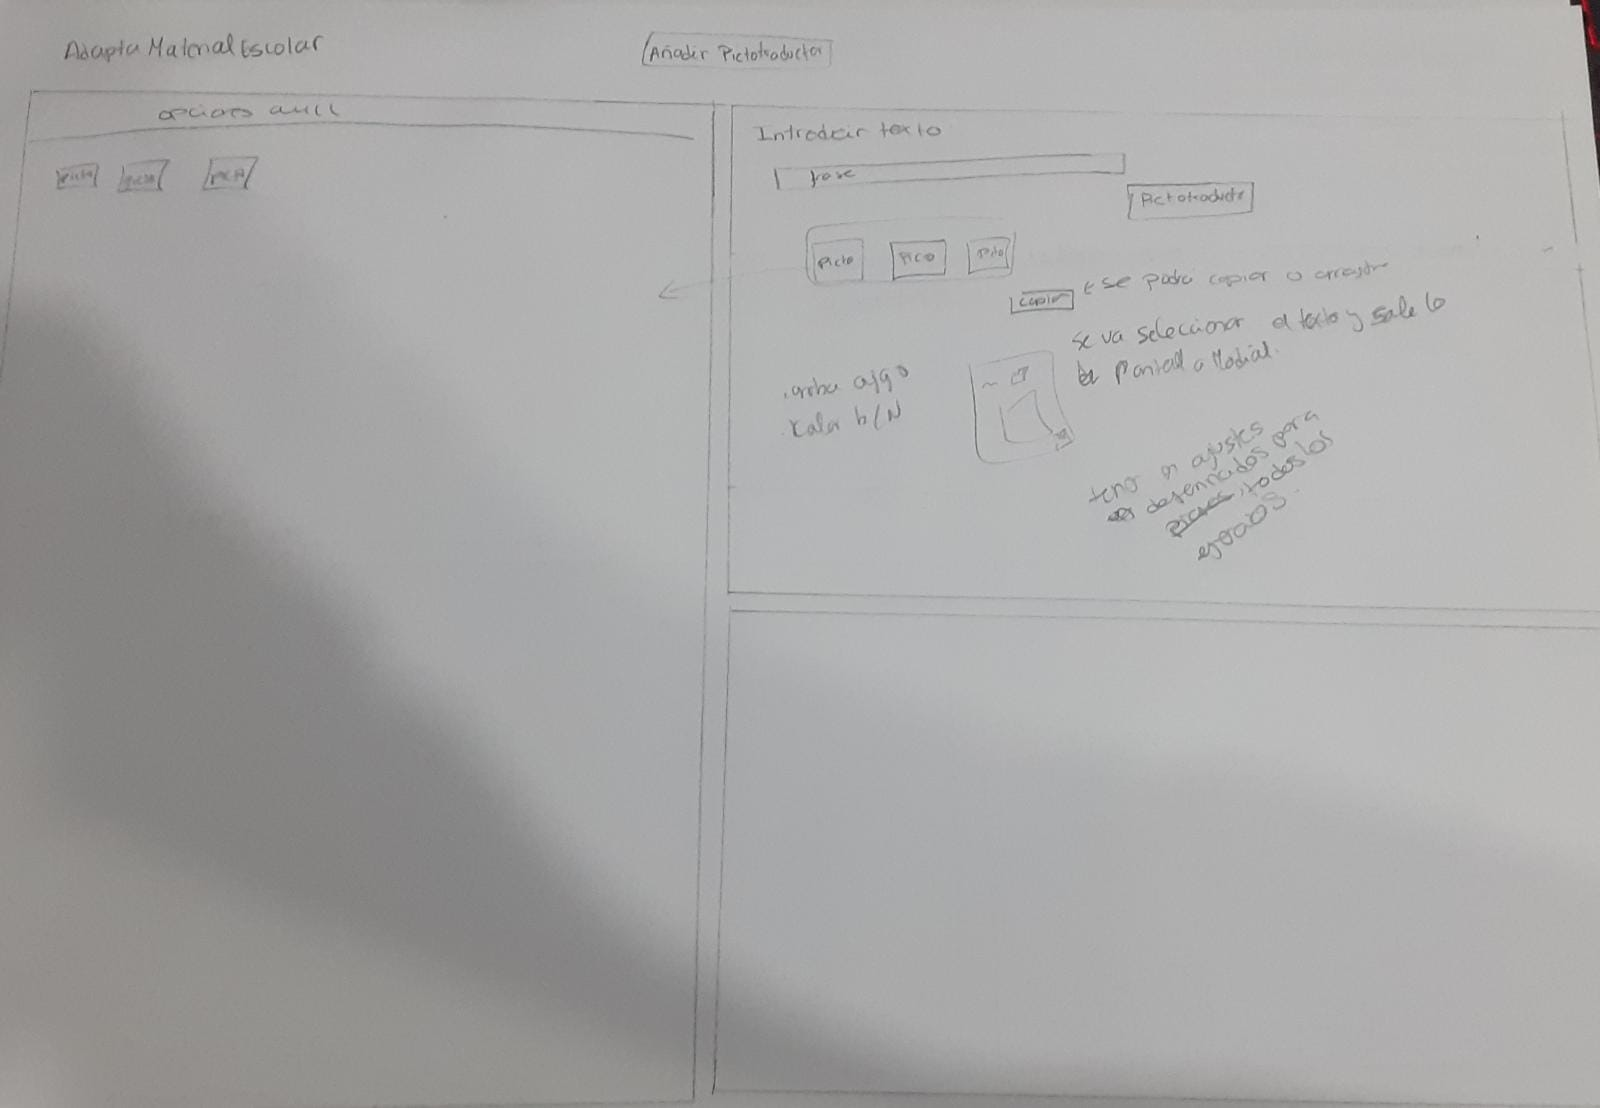
\includegraphics[width=0.6\textwidth]{Diseño/Dunia/picto.jpeg}
    \caption{Diseño de pictotraductor de Dunia.}
    \label{dunia3}
  \end{figure}

  \begin{figure}[ht!]
    \centering
    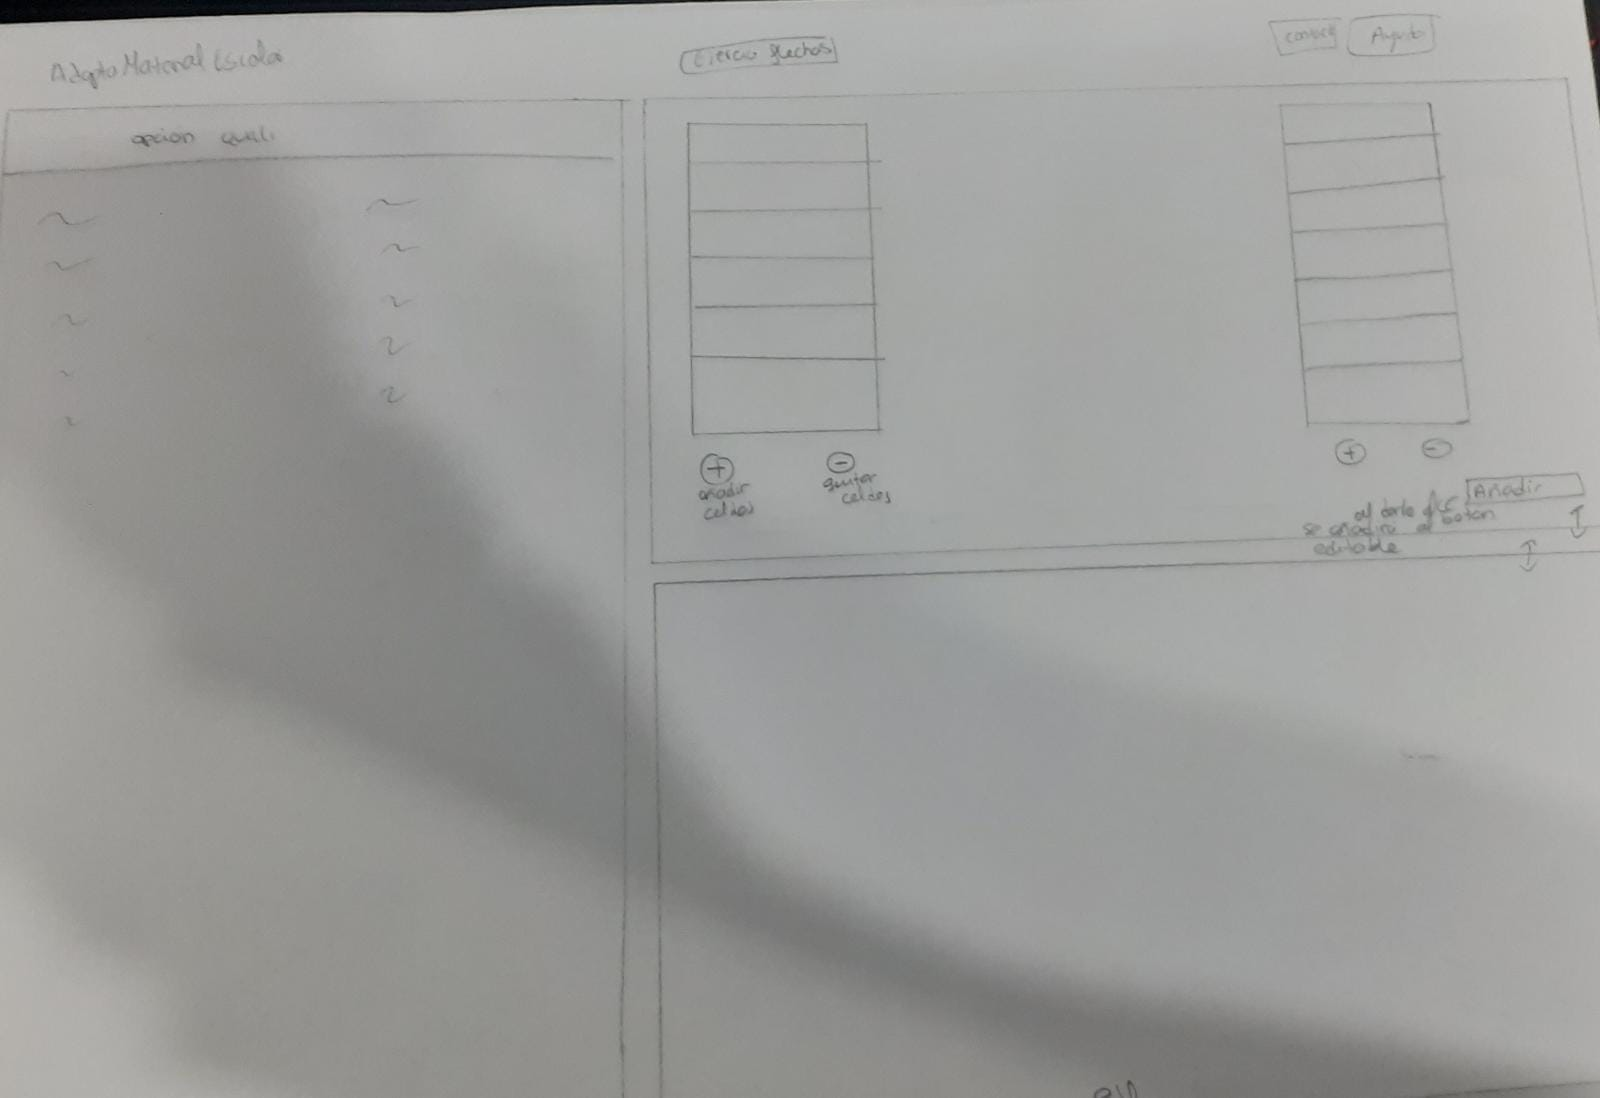
\includegraphics[width=0.7\textwidth]{Diseño/Dunia/flechas.jpeg}
    \caption{Diseño de ejercicios de flechas de Dunia.}
    \label{dunia4}
  \end{figure}

  \begin{figure}[ht!]
    \centering
    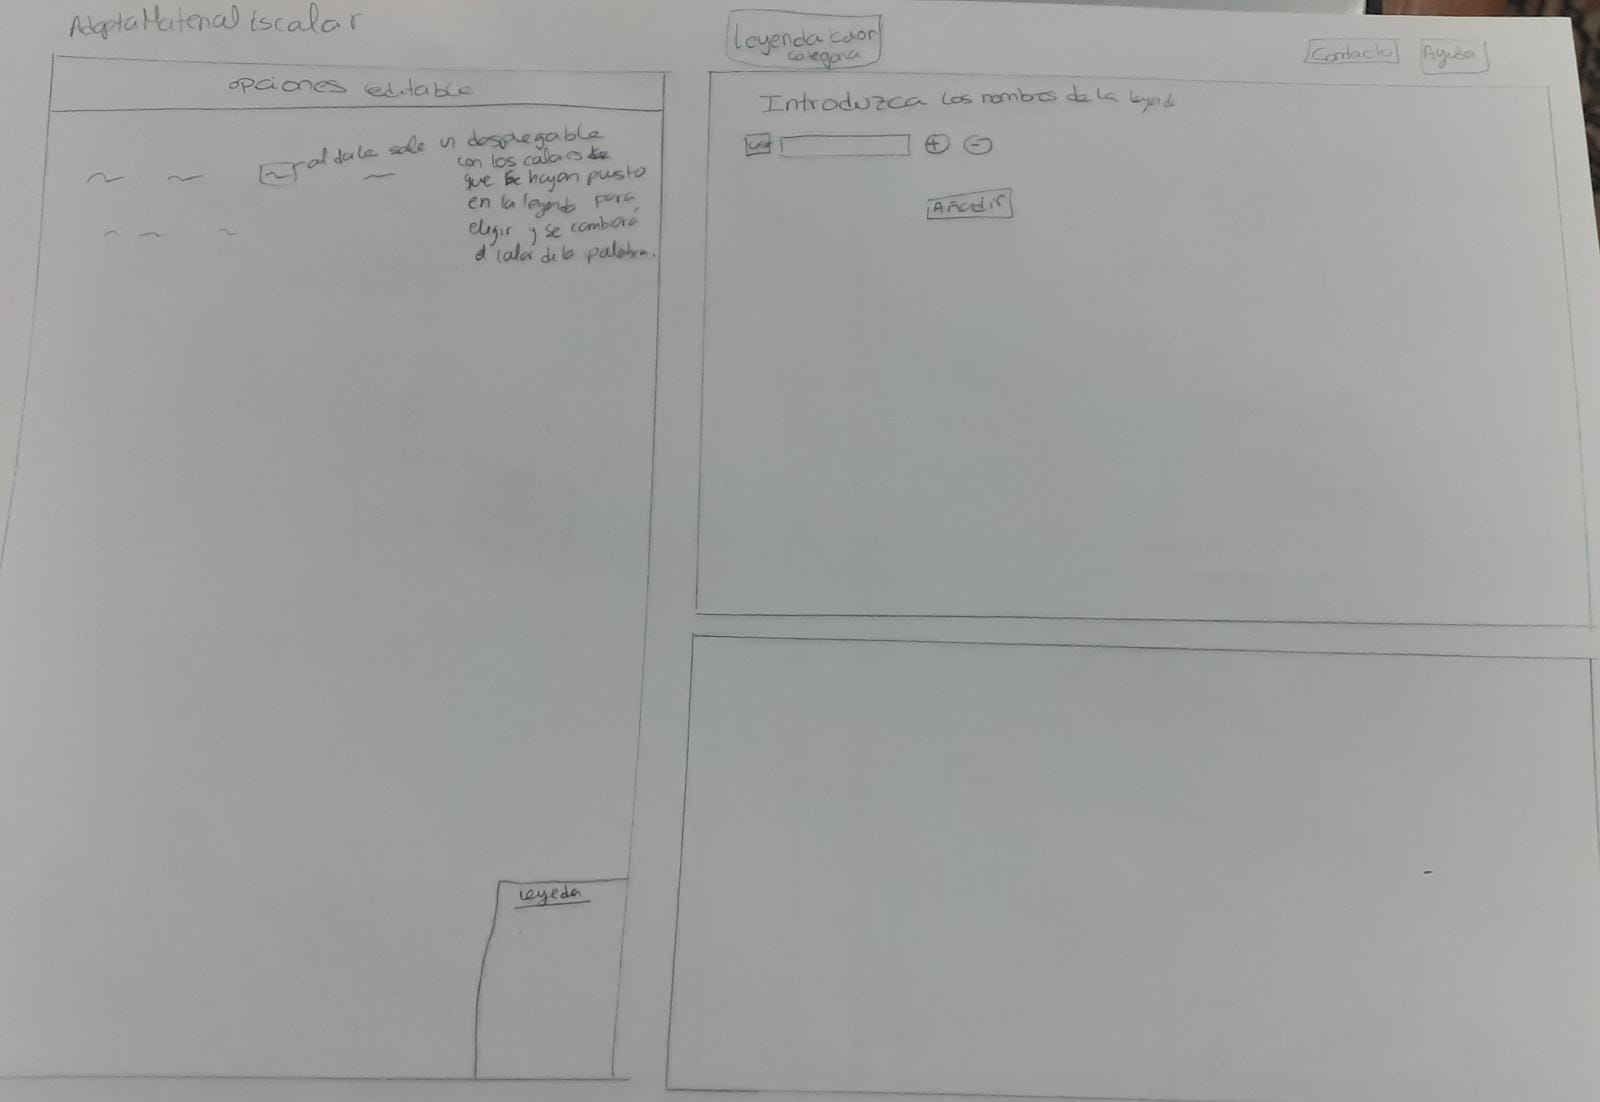
\includegraphics[width=0.7\textwidth]{Diseño/Dunia/leyendaColor.jpeg}
    \caption{Diseño de leyenda de colores de Dunia.}
    \label{dunia5}
  \end{figure}

  \begin{figure}[ht!]
    \centering
    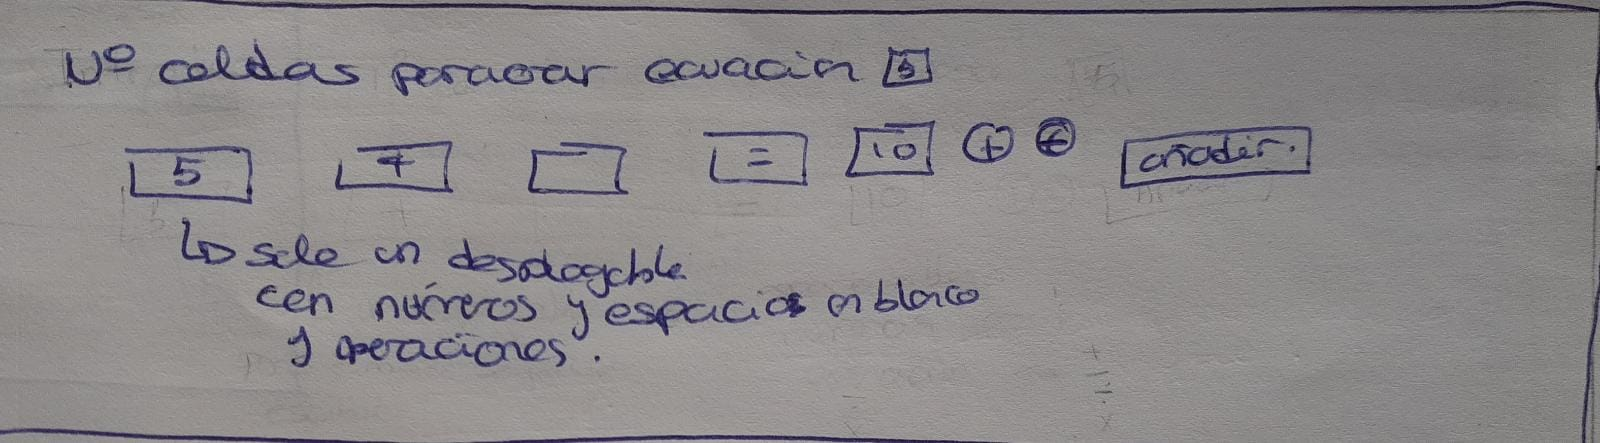
\includegraphics[width=0.7\textwidth]{Diseño/Dunia/hueco.jpeg}
    \caption{Diseño de ejercicios matemáticas de huecos de Dunia.}
    \label{dunia6}
  \end{figure}